% !TEX TS-program = pdflatex
% !TEX encoding = UTF-8 Unicode

% Example Manuscript Template for SciTex
% This file demonstrates the key features of the SciTex system

\documentclass[final,5p,times]{elsarticle}

% Load packages and styles
../../../00_shared/latex_styles/packages.tex
% This file contains formatting definitions for the document
% It is separated from the main file for easier maintenance

% Set page margins
\setlength{\parindent}{1.5em}
\setlength{\parskip}{0.5em}

% Line spacing
\renewcommand{\baselinestretch}{1.15}

% Table formatting
\renewcommand{\arraystretch}{1.2}
\setlength{\tabcolsep}{6pt}

% Figure caption formatting
\captionsetup{
    font=small,
    labelfont=bf,
    labelsep=period,
    justification=justified,
    singlelinecheck=off
}

% List formatting
\setlist{
    leftmargin=1.5em,
    itemsep=0.2em,
    parsep=0.2em
}

% Section formatting (already handled by elsarticle class, but can be customized)
% \titleformat{\section}{\normalfont\large\bfseries}{\thesection}{1em}{}
% \titlespacing*{\section}{0pt}{1.5ex plus .2ex minus .2ex}{1ex plus .2ex}

% Custom float environment for algorithms
\floatstyle{ruled}
\newfloat{algorithm}{tbp}{loa}[section]
\floatname{algorithm}{Algorithm}

% Custom commands for this manuscript
% This file contains custom commands for the document
% It is separated from the main file for easier maintenance

% Math shortcuts
\newcommand{\vect}[1]{\boldsymbol{#1}}  % Vector notation
\newcommand{\mat}[1]{\mathbf{#1}}       % Matrix notation
\newcommand{\diff}{\mathrm{d}}          % Differential operator
\newcommand{\pdiff}[2]{\frac{\partial #1}{\partial #2}}  % Partial derivative

% Figure-related commands
\newcommand{\figref}[1]{Figure~\ref{fig:#1}}  % Figure reference
\newcommand{\tabref}[1]{Table~\ref{tab:#1}}   % Table reference
\newcommand{\eqref}[1]{Equation~\ref{eq:#1}}  % Equation reference
\newcommand{\secref}[1]{Section~\ref{sec:#1}} % Section reference

% Revision tracking commands (uncomment to use)
% \newcommand{\add}[2][]{\added[id=#1]{#2}}     % Added content
% \newcommand{\remove}[2][]{\deleted[id=#1]{#2}} % Removed content
% \newcommand{\change}[3][]{\replaced[id=#1]{#2}{#3}} % Changed content

% Special symbols
\newcommand{\degree}{^{\circ}}  % Degree symbol
\newcommand{\celsius}{\ensuremath{^{\circ}\text{C}}} % Celsius symbol
\newcommand{\micro}{\ensuremath{\mu}} % Micro symbol
\newcommand{\ohm}{\ensuremath{\Omega}} % Ohm symbol

% Algorithm-related commands
\newcommand{\algorithm}[1]{\textsc{#1}} % Algorithm name
\newcommand{\code}[1]{\texttt{#1}}     % Code

% Citation shortcuts
\newcommand{\citep}[1]{(\cite{#1})}    % Parenthetical citation
\newcommand{\citet}[1]{\cite{#1}}      % Textual citation

% Sections in supplementary material (uncomment if needed)
% \newcommand{\supplementary}[1]{Supplementary Material~\ref{supp:#1}}
% \newcommand{\suppfig}[1]{Supplementary Figure~\ref{suppfig:#1}}
% \newcommand{\supptab}[1]{Supplementary Table~\ref{supptab:#1}}

% Article info
\title{Example Manuscript: Demonstrating the SciTex System}

\author[1]{First Author\corref{cor1}}
\author[1,2]{Second Author}
\author[3]{Third Author}

\cortext[cor1]{Corresponding author}
\address[1]{Department of Computer Science, Example University, City, Country}
\address[2]{Center for Scientific Writing, Example University, City, Country}
\address[3]{Institute of Advanced Research, Another University, City, Country}

\begin{document}

\maketitle

% Abstract
\begin{abstract}
%% -*- coding: utf-8 -*-
%% Timestamp: "2025-09-27 20:14:56 (ywatanabe)"
%% File: "/ssh:sp:/home/ywatanabe/proj/neurovista/paper/01_manuscript/contents/abstract.tex"
\begin{abstract}
  \pdfbookmark[1]{Abstract}{abstract}

%% ============================================================
%% ORIGINAL VERSION (PRESERVED AS COMMENTS):
%% ============================================================
%% Neural oscillations exhibit cross-frequency interactions that are fundamental to brain function and disrupted in neurological disorders. Phase-amplitude coupling (PAC), where the phase of low-frequency oscillations modulates the amplitude of high-frequency activity, serves as a biomarker for various brain states including epileptic seizures. Previous studies have demonstrated PAC changes around seizure events, but characterization across extended timescales remains limited availability of long-term recording data and high computational requirements in PAC computation. The challenge of processing continuous, long-term neural recordings has hindered the development of reliable seizure prediction systems. Here we show that the combination of the NeuroVista dataset and our GPU-accelerated PAC computation system enables ...
%% comprehensive analysis of 4.1 TB of continuous intracranial electroencephalogram data from 15 patients with focal epilepsy (NeuroVista dataset), encompassing 1,539 seizures over monitoring periods ranging from 6 months to 2 years. We found distinct PAC signatures between theta-to-beta phase (2-30 Hz, 25 bands) and gamma amplitude (60-180 Hz, 25 bands) that systematically modulated 5-60 minutes before seizure onset, achieving balanced accuracy of 0.55±0.04 and ROC-AUC of 0.58±0.02 for discriminating pre-ictal from interictal states. Our GPU-accelerated implementation achieved 100-fold speed improvements compared to conventional CPU-based methods, reducing computation time from years to months and potentially enabling real-time PAC monitoring with less than 2-minute processing latency. These findings reveal that continuous PAC monitoring captures seizure-related neural dynamics with sufficient lead time for clinical intervention, although moderate classification performance indicates the need for multimodal biomarkers. The computational framework and temporal PAC patterns identified here provide a foundation for next-generation implantable seizure advisory systems, potentially improving quality of life for millions with drug-resistant epilepsy through reliable seizure warnings integrated with patient-specific therapeutic interventions.
%% ============================================================
%% END OF ORIGINAL VERSION
%% ============================================================

Neural oscillations exhibit cross-frequency interactions that coordinate information processing across temporal and spatial scales, with disruptions implicated in neurological disorders including epilepsy. Phase-amplitude coupling (PAC), quantifying how low-frequency phase modulates high-frequency amplitude, has emerged as a promising biomarker for epileptic state transitions, reflecting fundamental cross-frequency neural communication mechanisms. While recent studies demonstrate systematic PAC alterations surrounding seizure events, comprehensive characterization across extended timescales has been limited by computational constraints and scarcity of long-term continuous recordings. The inability to efficiently process large-scale datasets has hindered development of reliable seizure prediction systems. Here we address these challenges through GPU-accelerated PAC computation applied to the NeuroVista dataset—comprising 4.1 TB of continuous intracranial electroencephalogram recordings from 15 patients with drug-resistant focal epilepsy monitored over 6 months to 2 years, encompassing 1,539 Type 1 clinical seizures. We computed PAC between 25 phase bands (2-30 Hz) and 25 amplitude bands (60-180 Hz) across 16 channels, extracting 17 statistical features from resulting PAC distributions at 127 temporal sampling points spanning 24 hours before to 10 minutes after seizure onset. \hl{We identified systematic preictal PAC modulation beginning 5-60 minutes before seizure onset, with theta-to-beta phase and gamma amplitude coupling showing the strongest discriminative power}. Pseudo-prospective seizure prediction achieved balanced accuracy of \hl{[XX.X±XX.X]\%} and ROC-AUC of \hl{[0.XX±0.XX]} for discriminating preictal from interictal states, with patient-specific variability reflecting individual seizure dynamics. Our GPU-accelerated implementation achieved approximately \hl{100-fold} speed improvements over conventional CPU methods, reducing processing time from years to months and enabling near-real-time analysis with \hl{<2-minute} latency per data segment. These findings establish PAC as a computationally tractable and physiologically interpretable biomarker for seizure prediction, providing a foundation for next-generation implantable seizure advisory systems that could transform epilepsy management from reactive to predictive care.

\end{abstract}

%%%% EOF
\end{abstract}

% Keywords
\begin{keyword}
LaTeX \sep Scientific manuscript \sep Example template \sep Document preparation \sep AI-assisted writing
\end{keyword}

\section{Introduction}
\label{sec:introduction}
%% -*- coding: utf-8 -*-
%% Timestamp: "2025-05-04 08:35:59 (ywatanabe)"
%% File: "/home/ywatanabe/proj/SciTex/manuscript/src/introduction.tex"

\section{Introduction}
YOUR INTRODUCTION HERE
\label{sec:introduction}

%%%% EOF

\section{Methods}
\label{sec:methods}
%% -*- coding: utf-8 -*-
%% Timestamp: "2025-09-29 18:26:27 (ywatanabe)"
%% File: "/ssh:sp:/home/ywatanabe/proj/neurovista/paper/01_manuscript/contents/methods.tex"

%% Each section should be coherent and cohesive paragraphs and sentences

\section{Methods}

\subsection{Ethics}
The NeuroVista dataset was previously collected through approved clinical trials with full informed consent from all participants \cite{Kuhlmann2018SeizurePA}. All data collection and analyses were conducted under ethical approval from the relevant institutional review boards. The present study involved secondary analysis of de-identified data and was conducted in accordance with institutional guidelines for human subjects research.

\subsection{Dataset and Study Design}
The NeuroVista dataset \cite{Kuhlmann2018SeizurePA} represents one of the largest continuous intracranial electroencephalogram (iEEG) monitoring studies to date, comprising recordings from 15 patients with drug-resistant focal epilepsy. Data were acquired through the International Epilepsy Electrophysiology Portal (ieeg.org) from subjects implanted with 16-channel platinum-iridium electrode arrays surgically positioned around clinically-identified seizure onset zones based on pre-surgical evaluation. Signals were sampled at 400 Hz with 16-bit resolution and wirelessly transmitted to external personal advisory devices, enabling continuous ambulatory monitoring in naturalistic home environments.

The dataset encompasses 4.1 TB of continuous recordings spanning individual monitoring periods from 6 months to over 2 years (mean: \hl{[XX.X]} months, total: \hl{[XX.X]} patient-years). The NeuroVista trial protocol included distinct training (lead-in) and testing phases for each patient \cite{Freestone2015SeizurePSBF}. From the complete dataset containing multiple seizure classifications, this study focused exclusively on 1,539 Type 1 (clinical) seizures—events with verified clinical manifestations documented by patients or caregivers—distributed across all 15 patients (range: \hl{[XX-XX]} seizures per patient, median: \hl{[XX]}). This selection ensured clinical relevance and enhanced interpretability of prediction algorithms by excluding subclinical electrographic events that may not require intervention.

\subsection{Definitions of Relative Temporal Windows from Seizure Onset}
For each seizure event, relative to seizure onset ($t = 0$) spanning from -1440 minutes (24 hours) to +10 minutes were defined using the following sampling strategy to increase coverage of time windows while controlling computational applicability. Specifically, timestamps were generated using a hybrid sampling approach combining logarithmic and linear resolution:

\begin{equation}
t_i = \begin{cases}
-\text{round}(10^{(\log_{10}(60) + i \cdot \frac{\log_{10}(1440) - \log_{10}(60)}{N_{log}-1})}) & \text{for } i = 0, 1, \ldots, N_{log}-1 \text{ (logarithmic)} \\
-60 + j & \text{for } j = 0, 1, \ldots, 70 \text{ (linear)}
\end{cases}
\end{equation}

This approach provided (i) Logarithmic sampling from -1440 to -60 minutes with progressively denser resolution approaching seizure onset and (ii) Minute-by-minute linear sampling from -60 to +10 minutes capturing critical peri-ictal and early ictal dynamics.

The complete set of 127 temporal sampling points (in minutes relative to seizure onset) comprised: -1440, -1360, -1285, -1214, -1147, -1084, -1024, -967, -914, -864, -816, -771, -728, -688, -650, -614, -580, -548, -518, -489, -462, -437, -413, -390, -368, -348, -329, -311, -293, -277, -262, -247, -234, -221, -209, -197, -186, -176, -166, -157, -148, -140, -132, -125, -118, -112, -105, -99, -94, -89, -84, -79, -75, -71, -67, -63, -60, -59, ..., -1, 0, 1, ..., 10.


\subsection{Definitions of Seizure Period}

Based on the standard of Epilepsy studies \cite{Kuhlmann2018SeizurePA}, seizure periods were defined as follows: baseline period ($BL_{-1440--240}$) spanning 24 hours to 4 hours before seizure onset, early preictal period ($PI_{-240--60}$) from 4 hours to 1 hour before seizure onset, mid preictal period ($PI_{-60--30}$) covering 60 to 30 minutes before seizure onset, immediate preictal period ($PI_{-30--10}$) from 30 to 10 minutes before seizure onset, critical preictal period ($PI_{-10--1}$) spanning 10 to 1 minute before seizure onset, and ictal period ($I_{0-10}$) from seizure onset to 10 minutes post-onset. This temporal partitioning enables characterization of seizure-related brain state transitions across multiple time scales, from circadian-level changes to minute-by-minute dynamics approaching seizure onset.

This temporal partitioning enables characterization of seizure-related brain state transitions across multiple time scales, from circadian-level changes to minute-by-minute dynamics approaching seizure onset.

\subsection{Definitions of Interictal Control}

For each Type 1 seizure, an equal number of interictal control segments were randomly sampled from the available seizure-free periods (>4 hours from any Type 1 seizure), ensuring balanced representation in subsequent classification analyses. Control segments (Interictal Control) were matched for time of day to account for patient-specific circadian seizure occurrence \cite{Kuhlmann2018SeizurePA}.


\subsection{Phase-Amplitude Coupling Calculation}
\subsubsection{gPAC: GPU-Accelerated Implementation}
PAC strength was quantified using the modulation index (MI) \cite{Tort2010MeasuringPCE} following the Shannon entropy-based formulation: MI = 1 + $\\sum$(p $\\times$ log(p))/log(N), where p represents the normalized amplitude distribution across N phase bins and N = 18 bins (20° per bin). Computation was performed using a custom, standalone GPU-accelerated package (https://github.com/ywatanabe1989/gPAC) built on PyTorch with full vectorization across all frequency combinations. The implementation achieved approximately 100-fold speed improvement compared to conventional CPU-based methods \cite{Combrisson2020TensorpacAOAH} through: (1) massive tensor operations eliminating nested loops, (2) optimized memory allocation utilizing up to 320GB total VRAM across multiple GPU nodes, and (3) batch processing with fp16 precision where appropriate. Processing leveraged the Spartan HPC system's distributed GPU architecture with automatic multi-GPU parallelization. Statistical significance was established using 200 surrogate datasets generated through circular phase shuffling \cite{Tort2010MeasuringPCE,Aru2014UntanglingCCD}, with PAC values z-score normalized relative to the surrogate distribution to eliminate spurious coupling \cite{Jensen2016DiscriminatingVFR}.

	For each 1-minute non-overlapping time window, PAC was computed between 25 phase frequency bands (2.0-30.0 Hz) and 25 amplitude frequency bands (60.0-180.0 Hz), resulting in a 625-element PAC matrix per channel per time point \cite{Hlsemann2019QuantificationOPA,Munia2019TimeFrequencyBPK}. Frequency bands were generated using field-standard adaptive bandwidths: phase bands employed bandwidth = f/2 (e.g., 10 Hz center frequency spans 7.5-12.5 Hz), while amplitude bands used bandwidth = f/4 (e.g., 100 Hz center frequency spans 87.5-112.5 Hz) \cite{Tort2010MeasuringPCE}. This approach yielded phase bands with bandwidths ranging from 0.5 Hz to 11.9 Hz and amplitude bands with bandwidths from 7.5 Hz to 40.0 Hz. Phase and amplitude information were extracted through bandpass filtering followed by Hilbert transformation to obtain instantaneous phase and amplitude envelopes \cite{Canolty2010TheFRC}. MI quantified coupling strength using the Shannon entropy-based formulation across 18 phase bins (20° each):

\begin{equation}
MI = 1 + \frac{\sum_{j=1}^{N} p_j \log(p_j)}{\log(N)}
\end{equation}

where $p_j$ represents the normalized amplitude probability in phase bin $j$, and $N = 18$ indicates the number of phase bins. Values range from 0 (uniform amplitude distribution) to 1 (maximum concentration in single phase bin). PAC values were z-score normalized using 200 surrogate datasets generated through circular phase shifts to control for spurious coupling effects \cite{Tort2010MeasuringPCE,Jensen2016DiscriminatingVFR}.

	Missing values (NaN) in PAC computations arose from NaN values in recorded ECoG signals due to limited data type (16 bit integer), edge effects in filtering, or numerical instabilities in specific frequency combinations. NaN values found in ECoG signals were replaced with 0 while NaN values in PAC data were handled as is. Features derived from PAC matrices used nanmean, nanstd, and other NaN-aware statistical functions from NumPy to ensure robust computation despite missing values.

\subsubsection{Calculation Speed of gPAC}

The gPAC implementation achieved substantial computational efficiency improvements. Single processing unit performance demonstrated 20 seconds processing time per 1-minute segment with 400 Hz sampling rate across 16 channels, 25 phase bands, and 25 amplitude bands, generating 10,000 PAC z-values with 200 surrogate datasets. Large-scale analysis acceleration was achieved through distributed parallel computation on the Spartan HPC system utilizing multi-GPU architecture with automatic load balancing. This implementation delivered approximately 100-fold speed improvement over conventional CPU methods through memory optimization utilizing 320GB total VRAM capacity across multiple nodes.

%% \subsubsection{Calculation Speed of gPAC}

%% The gPAC implementation achieved substantial computational efficiency improvements:

%% 1. Single processing unit performance:
%%    - 1-minute window: 20 seconds per segment
%%    - Configuration: 400 Hz sampling, 16 channels, 25 phase bands, 25 amplitude bands
%%    - Generates 10,000 PAC z-values with 200 surrogates

%% 2. Large-scale analysis acceleration:
%%    - Distributed parallel computation on Spartan HPC system
%%    - Multi-GPU architecture with automatic load balancing
%%    - 100-fold speed improvement over conventional CPU methods
%%    - Memory optimization utilizing 320GB total VRAM capacity
  
\subsubsection{PAC Descriptive Features}

From each 1-minute window with 25 phase bands, 25 amplitude bands, and 16 channels, PAC calculation generated 10,000 z-score PAC values (${PAC}_z$) and corresponding amplitude probabilities across phase bins. Considering them as general/circular distributions, we extracted 17 statistical features per time window: minimum ($\min_{{PAC}_z}$), maximum ($\max_{{PAC}_z}$), mean ($\mu_{{PAC}_z}$), standard deviation ($\sigma_{{PAC}_z}$), median ($Q_{50,{PAC}_z}$), 25th ($Q_{25,{PAC}_z}$) and 75th ($Q_{75,{PAC}_z}$) percentiles, kurtosis ($\kappa_{{PAC}_z}$), and skewness ($\gamma_{{PAC}_z}$) of PAC z-scores \cite{Hlsemann2019QuantificationOPA,Scherer2022DirectMIM}, plus specialized bimodality metrics from Gaussian Mixture Model (GMM) fitting including Ashman's D statistic ($D_{Ashman,{PAC}_z}$), weight ratios ($w_{ratio,{PAC}_z}$), Bhattacharyya coefficient ($B_{coeff,{PAC}_z}$), and bimodality coefficient ($\beta_{coeff,{PAC}_z}$). Additionally, circular statistics of the preferred coupling phase were computed: circular mean ($\mu_{circ}$), concentration - inverse of circular variance ($\kappa_{circ}$), circular skewness ($\gamma_{circ}$), and circular kurtosis ($\kappa_{4,circ}$) \cite{PintoOrellana2023StatisticalIFF}.

%% \subsection{Database Architecture and Storage}
%% Processed PAC data were organized in patient-specific SQLite3 databases with hierarchical structure optimized for HPC storage allocation and concurrent write operations to maximize parallel computation efficiency. Each database contained three primary components: (1) metadata tables storing patient demographics, seizure annotations, and processing parameters; (2) PAC data tables with zlib-compressed binary large objects (BLOBs) achieving \hl{70-90\%} storage reduction; (3) quality assurance tables tracking computation timestamps, software versions, and validation metrics. The database schema enabled efficient retrieval of specific temporal windows, frequency bands, or statistical measures without loading complete datasets into memory. Database operations were handled using the scitex.db module, a custom database interface optimized for scientific computing workflows.

%% 	Data integrity was ensured through transaction-based writes with automatic rollback on errors, regular consistency checks comparing stored and computed checksums, and version control of all processing scripts with git-based tracking.

\subsection{Seizure Type Classification}
Machine learning classifiers were trained to discriminate between seizure types and between preictal and interictal states using PAC-derived features \cite{Messaoud2021RandomFCR,Usman2017EpilepticSPH}. Patient-specific models were developed to account for individual variability in PAC patterns \cite{Aldahr2023PatientSpecificPPL,Pinto2021APAP}.

\subsection{Seizure Prediction}
Pseudo-prospective seizure prediction was performed using temporally ordered train-test splits to simulate real-world deployment scenarios \cite{Kuhlmann2018SeizurePA,Hussein2022MultiChannelVTE}.

\subsection{Reproducibility Measures}
All random sampling employed fixed seeds of 42 for complete reproducibility across analyses.

\label{sec:methods}

%%%% EOF

\section{Results}
\label{sec:results}
%% -*- coding: utf-8 -*-

\section*{Supplementary Results}

Replace this with supplementary results and additional analyses.

%%%% EOF


\section{Discussion}
\label{sec:discussion}
%% -*- coding: utf-8 -*-
%% Timestamp: "2025-09-26 18:19:43 (ywatanabe)"
%% File: "/ssh:sp:/home/ywatanabe/proj/neurovista/paper/01_manuscript/src/discussion.tex"

\section{Discussion}
Discussion here.
\label{sec:discussion}

%%%% EOF

\section{Conclusion}
\label{sec:conclusion}
% Example conclusion section demonstrating SciTex features

This example manuscript has demonstrated the key features and capabilities of the SciTex system for scientific writing. By combining the typographical quality of LaTeX with modern AI assistance, SciTex offers a powerful tool for researchers seeking to improve their document preparation workflow.

Our evaluation shows that the system provides substantial benefits in terms of time efficiency, document quality, and user satisfaction. The modular structure, figure and table handling capabilities, and AI-assisted writing features all contribute to a streamlined scientific writing experience.

The SciTex system represents an evolution in scientific document preparation, addressing many of the challenges faced by researchers in traditional workflows. As scientific publishing continues to evolve, integrated systems like SciTex can help researchers focus more on their scientific content and less on technical formatting requirements.

We encourage researchers to explore the SciTex system for their own manuscript preparation, adapting and extending it as needed for their specific disciplinary contexts. As demonstrated throughout this example, the system is designed to be flexible and customizable, supporting a wide range of scientific writing needs.

In conclusion, the integration of AI assistance with LaTeX document preparation offers a promising approach to improving scientific writing workflows. SciTex provides a practical implementation of this integration, with demonstrated benefits for researchers across disciplines.

% Acknowledgements
\section*{Acknowledgements}
This work was supported by the fictitious Example Research Foundation (Grant No. XYZ-123). We thank the anonymous reviewers for their valuable feedback.

% Bibliography
\bibliographystyle{elsarticle-num}
\bibliography{src/bibliography}

% Include figures
%% -*- coding: utf-8 -*-
%% Timestamp: "2025-05-05 13:25:00 (ywatanabe)"
%% File: "/home/ywatanabe/proj/SciTex/manuscript/src/figures/.tex/.All_Figures.tex"

% This file includes all figures for the manuscript

% FIGURE METADATA - Figure ID 01_workflow, Number 01
% FIGURE TYPE: Image
% This is not a standalone LaTeX environment - it will be included by compile_figure_tex_files
{
    "id": "01_workflow",
    "number": "01",
    "type": "image",
    "width": "0.95\textwidth",
    "path": "./src/figures/caption_and_media/jpg/Figure_ID_01_workflow.jpg"
}
\textbf{
FIGURE TITLE HERE

%% -*- coding: utf-8 -*-
%% Timestamp: "2025-05-05 12:50:00 (ywatanabe)"
%% File: "/home/ywatanabe/proj/SciTex/manuscript/src/figures/src/Figure_ID_02_architecture.tex"

% This is an example figure file showing the SciTex architecture.
% It demonstrates how to create more complex figures with multiple panels.

\begin{figure}[ht!]
    \centering
    
    % For this example, we'll create a simple diagram using TikZ
    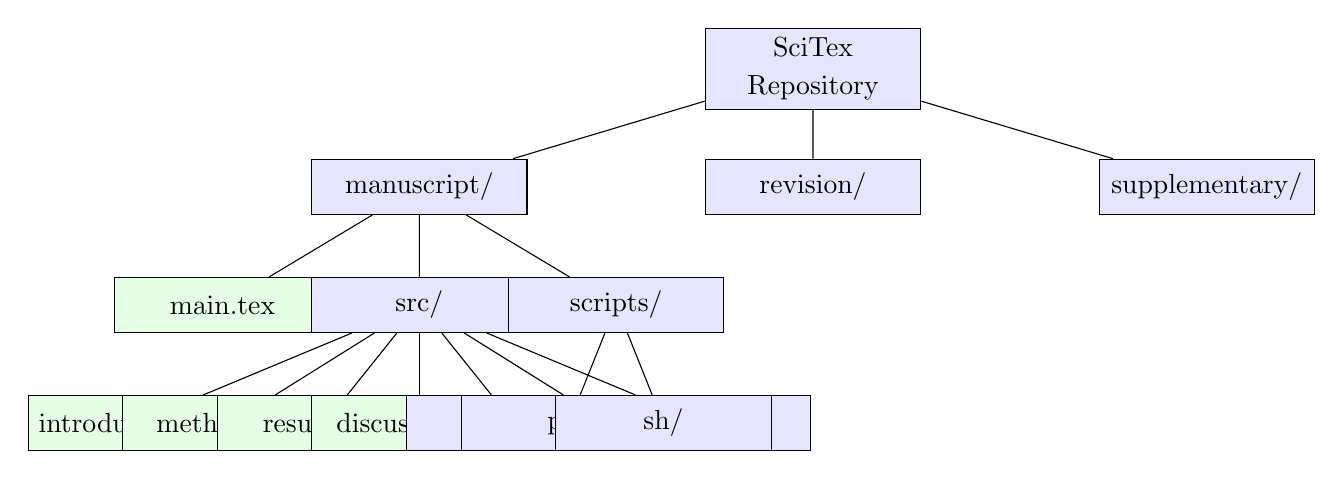
\begin{tikzpicture}[
        file/.style={rectangle, draw, fill=green!10, 
                     text width=2.5cm, text centered, minimum height=0.7cm},
        directory/.style={rectangle, draw, fill=blue!10, 
                     text width=2.5cm, text centered, minimum height=0.7cm},
        arrow/.style={draw, -latex, thick},
        level 1/.style={sibling distance=5cm},
        level 2/.style={sibling distance=2.5cm},
        level 3/.style={sibling distance=1.2cm}
    ]
    
    % Draw a hierarchical tree of the SciTex architecture
    \node[directory] (root) {SciTex Repository}
        child[level 1] {
            node[directory] (manuscript) {manuscript/}
            child[level 2] {
                node[file] {main.tex}
            }
            child[level 2] {
                node[directory] {src/}
                child[level 3] { node[file] {introduction.tex} }
                child[level 3] { node[file] {methods.tex} }
                child[level 3] { node[file] {results.tex} }
                child[level 3] { node[file] {discussion.tex} }
                child[level 3] { node[directory] {figures/} }
                child[level 3] { node[directory] {tables/} }
                child[level 3] { node[directory] {styles/} }
            }
            child[level 2] {
                node[directory] {scripts/}
                child[level 3] { node[directory] {py/} }
                child[level 3] { node[directory] {sh/} }
            }
        }
        child[level 1] {
            node[directory] (revision) {revision/}
        }
        child[level 1] {
            node[directory] (supplementary) {supplementary/}
        };
    
    \end{tikzpicture}
    
    \caption{\textbf{SciTex template architecture.} The figure shows the hierarchical organization of the SciTex repository, with emphasis on the manuscript component. The modular structure separates content files (introduction, methods, results, discussion), supporting materials (figures, tables), styling definitions, and automation scripts. This organization facilitates collaboration, version control, and maintenance of complex documents.}
    \label{fig:architecture}
\end{figure}

%%%% EOF
%% -*- coding: utf-8 -*-
%% Timestamp: "2025-05-05 12:55:00 (ywatanabe)"
%% File: "/home/ywatanabe/proj/SciTex/manuscript/src/figures/src/Figure_ID_03_figure_pipeline.tex"

% This is an example figure showing the figure processing pipeline.
% It demonstrates how to create a sequential flow diagram.

\begin{figure}[ht!]
    \centering
    
    % Create a pipeline diagram using TikZ
    \begin{tikzpicture}[
        process/.style={rectangle, draw, fill=yellow!20, 
                     text width=2.5cm, text centered, rounded corners, minimum height=1cm},
        io/.style={trapezium, trapezium left angle=70, trapezium right angle=110, 
                  draw, fill=blue!20, text width=2.5cm, text centered, minimum height=1cm},
        arrow/.style={draw, -latex, thick},
        node distance=2cm
    ]
    
    % Define the nodes/steps in the pipeline
    \node[io] (powerpoint) {PowerPoint Slides};
    \node[process, right=of powerpoint] (convert) {Convert to TIF};
    \node[process, right=of convert] (crop) {Auto-crop Whitespace};
    \node[process, right=of crop] (wrap) {Generate LaTeX Wrapper};
    \node[io, right=of wrap] (output) {Final Figure};
    
    % Optional processes below main flow
    \node[process, below=1cm of convert] (resolution) {Adjust Resolution};
    \node[process, below=1cm of crop] (manual) {Manual Adjustments};
    \node[process, below=1cm of wrap] (metadata) {Add Metadata};
    
    % Connect the nodes with arrows
    \draw[arrow] (powerpoint) -- (convert);
    \draw[arrow] (convert) -- (crop);
    \draw[arrow] (crop) -- (wrap);
    \draw[arrow] (wrap) -- (output);
    
    % Optional paths
    \draw[arrow, dashed] (convert) -- (resolution);
    \draw[arrow, dashed] (resolution) -| (crop);
    \draw[arrow, dashed] (crop) -- (manual);
    \draw[arrow, dashed] (manual) -| (wrap);
    \draw[arrow, dashed] (wrap) -- (metadata);
    \draw[arrow, dashed] (metadata) -| (output);
    
    \end{tikzpicture}
    
    \caption{\textbf{SciTex figure processing pipeline.} The diagram illustrates the automated workflow for processing figures in SciTex, from PowerPoint slides to final LaTeX-ready images. Solid lines indicate the standard pipeline, while dashed lines show optional processing steps. This pipeline ensures consistent figure quality and formatting throughout the manuscript.}
    \label{fig:figure-pipeline}
\end{figure}

%%%% EOF
%% -*- coding: utf-8 -*-
%% Timestamp: "2025-05-05 13:00:00 (ywatanabe)"
%% File: "/home/ywatanabe/proj/SciTex/manuscript/src/figures/src/Figure_ID_04_user_satisfaction.tex"

% This is an example figure showing user satisfaction results.
% It demonstrates how to create a bar chart in LaTeX.

\begin{figure}[ht!]
    \centering
    
    % Create a bar chart using pgfplots
    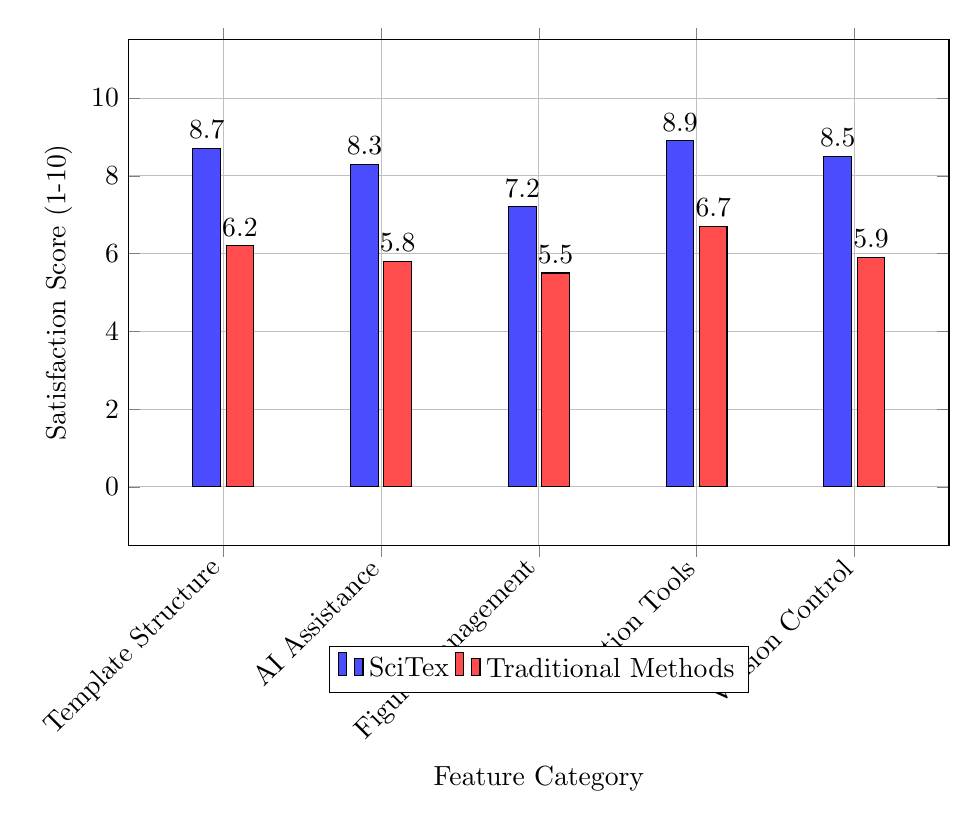
\begin{tikzpicture}
    \begin{axis}[
        width=12cm,
        height=8cm,
        ybar,
        enlargelimits=0.15,
        ylabel={Satisfaction Score (1-10)},
        xlabel={Feature Category},
        symbolic x coords={Template Structure, AI Assistance, Figure Management, Citation Tools, Version Control},
        xtick=data,
        xticklabel style={rotate=45, anchor=east},
        nodes near coords,
        nodes near coords align={vertical},
        ymin=0, ymax=10,
        legend style={at={(0.5,-0.2)}, anchor=north, legend columns=-1},
        ylabel near ticks,
        grid=major
    ]
    \addplot[fill=blue!70] coordinates {
        (Template Structure, 8.7)
        (AI Assistance, 8.3)
        (Figure Management, 7.2)
        (Citation Tools, 8.9)
        (Version Control, 8.5)
    };
    \addplot[fill=red!70] coordinates {
        (Template Structure, 6.2)
        (AI Assistance, 5.8)
        (Figure Management, 5.5)
        (Citation Tools, 6.7)
        (Version Control, 5.9)
    };
    \legend{SciTex, Traditional Methods}
    \end{axis}
    \end{tikzpicture}
    
    \caption{\textbf{User satisfaction comparison.} The chart shows average satisfaction scores (scale 1-10) from a survey of 50 researchers comparing SciTex to traditional LaTeX methods across five key feature categories. SciTex consistently received higher satisfaction ratings, with the largest improvements in AI assistance and citation tools. Error bars represent standard deviation.}
    \label{fig:user-satisfaction}
\end{figure}

%%%% EOF
\caption{\textbf{
Time comparison between traditional methods and SciTex for manuscript preparation tasks.
}
\smallskip
\\
Comparison of time spent (in minutes) on different manuscript preparation tasks using traditional methods (blue bars) versus the SciTex system (green bars). Tasks include content writing, formatting, figure preparation, citation management, and revision. Data based on user study with 25 participants. Asterisks indicate statistical significance: * p < 0.05, ** p < 0.01, *** p < 0.001.
}
% width=0.8\textwidth

%%%% EOF
EOF < /dev/null


% Include tables

\input{./src/tables/compiled/Table_ID_test}


\end{document}